\documentclass[a4paper]{report}
\usepackage[14pt]{extsizes}
\usepackage[utf8]{inputenc}
\usepackage[english,russian]{babel}
\usepackage[OT1]{fontenc}
\usepackage{setspace, amsmath}
\usepackage{amsfonts}
\usepackage{amssymb}
\usepackage[left=20mm, top=10mm, right=15mm, bottom=20mm, nohead, footskip=10mm]{geometry}
\usepackage{gensymb}

\usepackage{graphicx} 
\graphicspath{{images/}}
\DeclareGraphicsExtensions{.pdf,.png,.jpg}

\renewcommand{\theenumi}{\arabic{enumi}}
\renewcommand{\labelenumi}{\arabic{enumi}}
\renewcommand{\theenumii}{.\arabic{enumii}}
\renewcommand{\labelenumii}{\arabic{enumi}.\arabic{enumii}.}
\renewcommand{\theenumiii}{.\arabic{enumiii}}
\renewcommand{\labelenumiii}{\arabic{enumi}.\arabic{enumii}.\arabic{enumiii}.}
\usepackage{indentfirst}
\usepackage{fontspec}
\setmainfont{Times New Roman}

\begin{document}
\chapter{Изучение алгоритмов сжатия данных, в частности, сжатия
аудиоинформации.}
\section{Определение}
\textbf{Сжатие данных} — алгоритмическое обратимое преобразование данных, производимое с целью уменьшения занимаемого ими объёма. Применяется для более рационального использования устройств хранения и передачи данных.
\par Сжатие основано на устранении избыточности, содержащейся в исходных данных. Простейшим примером избыточности является повторение в тексте фрагментов (например, слов естественного или машинного языка). Подобная избыточность обычно устраняется заменой повторяющейся последовательности ссылкой на уже закодированный фрагмент с указанием его длины. Другой вид избыточности связан с тем, что некоторые значения в сжимаемых данных встречаются чаще других. Сокращение объёма данных достигается за счёт замены часто встречающихся данных короткими кодовыми словами, а редких — длинными (энтропийное кодирование). Сжатие данных, не обладающих свойством избыточности (например, случайный сигнал или белый шум, зашифрованные сообщения), принципиально невозможно без потерь.
\section{Принципы сжатия данных}
В основе любого способа сжатия лежит модель источника данных, или, точнее, модель избыточности. Иными словами, для сжатия данных используются некоторые априорные сведения о том, какого рода данные сжимаются. Не обладая такими сведениями об источнике, невозможно сделать никаких предположений о преобразовании, которое позволило бы уменьшить объём сообщения. Модель избыточности может быть статической, неизменной для всего сжимаемого сообщения, либо строиться или параметризоваться на этапе сжатия (и восстановления). Методы, позволяющие на основе входных данных изменять модель избыточности информации, называются адаптивными. Неадаптивными являются обычно узкоспециализированные алгоритмы, применяемые для работы с данными, обладающими хорошо определёнными и неизменными характеристиками. Подавляющая часть достаточно универсальных алгоритмов является в той или иной мере адаптивной.

Все методы сжатия данных делятся на два основных класса:
\begin{itemize}
\item Сжатие без потерь
\item Сжатие с потерями
\end{itemize}
При использовании сжатия без потерь возможно полное восстановление исходных данных, сжатие с потерями позволяет восстановить данные с искажениями, обычно несущественными с точки зрения дальнейшего использования восстановленных данных. Сжатие без потерь обычно используется для передачи и хранения текстовых данных, компьютерных программ, реже — для сокращения объёма аудио- и видеоданных, цифровых фотографий и т. п., в случаях, когда искажения недопустимы или нежелательны. Сжатие с потерями, обладающее значительно большей, чем сжатие без потерь, эффективностью, обычно применяется для сокращения объёма аудио- и видеоданных и цифровых фотографий в тех случаях, когда такое сокращение является приоритетным, а полное соответствие исходных и восстановленных данных не требуется. 
\section{Основные характеристики алгоритмов сжатия}
\subsection{Коэффициент сжатия}
\textbf{Коэффициент сжатия} — основная характеристика алгоритма сжатия. Она определяется как отношение объёма исходных несжатых данных к объёму сжатых данных, то есть: $k = \frac{S_o}{S_c}$, где $k$ - коэффициент сжатия, $S_o$ - объём исходных данных, а $S_c$ - объём сжатых. Таким образом, чем выше коэффициент сжатия, тем алгоритм эффективнее. Следует отметить:
\begin{itemize}
\item если k = 1, то алгоритм не производит сжатия, то есть выходное сообщение оказывается по объёму равным входному;
\item если k < 1, то алгоритм порождает сообщение большего размера, нежели несжатое, то есть, совершает «вредную» работу.
\end{itemize}
\subsection{Допустимость потерь}
Основным критерием различия между алгоритмами сжатия является описанное выше наличие или отсутствие потерь. В общем случае алгоритмы сжатия без потерь универсальны в том смысле, что их применение безусловно возможно для данных любого типа, в то время как возможность применения сжатия с потерями должна быть обоснована. Для некоторых типов данных искажения не допустимы в принципе. В их числе:
\begin{itemize}
\item символические данные, изменение которых неминуемо приводит к изменению их семантики: программы и их исходные тексты, двоичные массивы и т.п.;
\item жизненно важные данные, изменения в которых могут привести к критическим ошибкам: например, получаемые с медицинской измерительной аппаратуры или контрольных приборов летательных, космических аппаратов и т.п.;
\item многократно подвергаемые сжатию и восстановлению промежуточные данные при многоэтапной обработке графических, звуковых и видеоданных.
\end{itemize}
\subsection{Системные требования алгоритмов}
Различные алгоритмы могут требовать различного количества ресурсов вычислительной системы, на которых они реализованы:
\begin{itemize}
\item оперативной памяти (под промежуточные данные);
\item постоянной памяти (под код программы и константы);
\item процессорного времени.

\end{itemize}
В целом, эти требования зависят от сложности и «интеллектуальности» алгоритма. Общая тенденция такова: чем эффективнее и универсальнее алгоритм, тем большие требования к вычислительным ресурсам он предъявляет. Тем не менее, в специфических случаях простые и компактные алгоритмы могут работать не хуже сложных и универсальных. Системные требования определяют их потребительские качества: чем менее требователен алгоритм, тем на более простой, а следовательно, компактной, надёжной и дешёвой системе он может быть реализован.

Так как алгоритмы сжатия и восстановления работают в паре, имеет значение соотношение системных требований к ним. Нередко можно, усложнив один алгоритм, значительно упростить другой. Таким образом, возможны три варианта:
\subsubsection{Алгоритм сжатия требует больших вычислительных ресурсов, нежели алгоритм восстановления.}
Это наиболее распространённое соотношение, характерное для случаев, когда однократно сжатые данные будут использоваться многократно. В качестве примера можно привести цифровые аудио- и видеопроигрыватели.
\subsubsection{Алгоритмы сжатия и восстановления требуют приблизительно равных вычислительных ресурсов.}
Наиболее приемлемый вариант для линий связи, когда сжатие и восстановление происходит однократно на двух её концах (например, в цифровой телефонии).
\subsubsection{Алгоритм сжатия существенно менее требователен, чем алгоритм восстановления.}
Такая ситуация характерна для случаев, когда процедура сжатия реализуется простым, часто портативным, устройством, для которого объём доступных ресурсов весьма критичен, например, космический аппарат или большая распределённая сеть датчиков. Это могут быть также данные, распаковка которых требуется в очень малом проценте случаев, например запись камер видеонаблюдения.
\section{Кодирование аудиоданных}
\subsection{Принципы оцифровки звука}
\textbf{Цифровой звук} — это аналоговый звуковой сигнал, представленный посредством дискретных численных значений его амплитуды.

\textbf{Оцифровка звука} — технология осуществления замеров амплитуды звукового сигнала с определенным временным шагом и последующей записи полученных значений в численном виде.
Другое название оцифровки звука — аналогово-цифровое преобразование звука.

Оцифровка звука включает в себя два процесса:
\begin{itemize}
\item процесс дискретизации (осуществление выборки) сигнала по времени
\item процесс квантования по амплитуде.
\end{itemize}

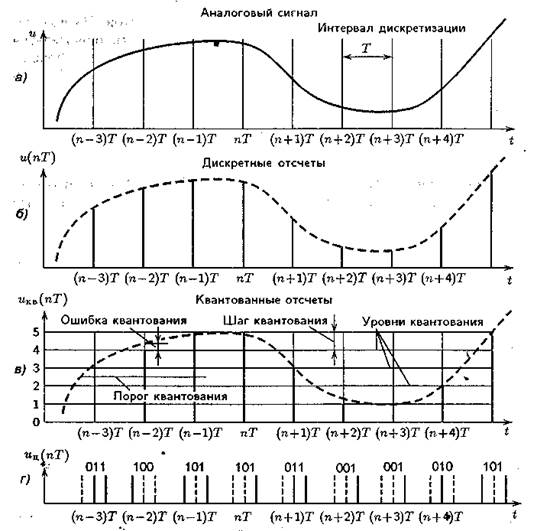
\includegraphics[scale=0.8]{Analog_to_digi}
{\centering\par{Рис. 1.4.1.1 Схема оцифровки звука}\\}
~
\subsubsection{Процесс дискретизации по времени}
\textbf{Процесс дискретизации по времени} — процесс получения значений сигнала, который преобразуется с определенным временным шагом — шагом дискретизации . Количество замеров величины сигнала, осуществляемых в единицу времени, называют частотой дискретизации или частотой выборки. Чем меньше шаг дискретизации, тем выше частота дискретизации и тем более точное представление о сигнале будет получено.
Это подтверждается теоремой Котельникова. Согласно ей, аналоговый сигнал с ограниченным спектром точно описуем дискретной последовательностью значений его амплитуды, если эти значения берутся с частотой, как минимум вдвое превышающей наивысшую частоту спектра сигнала. То есть, аналоговый сигнал, в котором находится частота спектра равная $F_m$, может быть точно представлен последовательностью дискретных значений амплитуды, если для частоты дискретизации $F_d$ выполняется: $F_d>2F_m$.
\par На практике это означает, что для того, чтобы оцифрованный сигнал содержал информацию о всем диапазоне слышимых частот исходного аналогового сигнала (20 Гц — 20 кГц) необходимо, чтобы выбранное значение частоты дискретизации составляло не менее 40 кГц.
\par Основная трудность оцифровки заключается в невозможности записать измеренные значения сигнала с идеальной точностью.
\subsubsection{Линейное квантование амплитуды}
Отведём для записи одного значения амплитуды сигнала в памяти компьютера $N$ бит. Значит, с помощью одного $N$-битного слова можно описать $2N$ разных положений. Пусть амплитуда оцифровываемого сигнала колеблется в пределах от −1 до 1 некоторых условных единиц. Представим этот диапазон изменения амплитуды — \textbf{динамический диапазон сигнала} — в виде $2N−1$ равных промежутков, разделив его на $2N$ уровней — \textbf{квантов}. Теперь, для записи каждого отдельного значения амплитуды, его необходимо округлить до ближайшего уровня квантования. Этот процесс носит название \textbf{квантования по амплитуде}.

\textbf{Квантование по амплитуде} — процесс замены реальных значений амплитуды сигнала значениями, приближенными с некоторой точностью. Каждый из $2^N$ возможных уровней называется \textbf{уровнем квантования}, а расстояние между двумя ближайшими уровнями квантования называется \textbf{шагом квантования}. Если амплитудная шкала разбита на уровни линейно, квантование называют линейным (однородным).
Точность округления зависит от выбранного количества $2N$ уровней квантования, которое, в свою очередь, зависит от количества бит $N$, отведенных для записи значения амплитуды. Число $N$ называют \textbf{разрядностью квантования}, а полученные в результате округления значений амплитуды числа — \textbf{отсчетами} или \textbf{семплами}. Принимается, что погрешности квантования, являющиеся результатом квантования с разрядностью 16 бит, остаются для слушателя почти незаметными. Этот способ оцифровки сигнала — дискретизация сигнала во времени в совокупности с методом однородного квантования — называется \textbf{импульсно-кодовой модуляцией, ИКМ (англ. Pulse Code Modulation — PCM)}.

Оцифрованный сигнал в виде набора последовательных значений амплитуды уже можно сохранить в памяти компьютера. В случае, когда записываются абсолютные значения амплитуды, такой формат записи называется PCM (Pulse Code Modulation). Стандартный аудио компакт-диск (CD-DA), применяющийся с начала 80-х годов, хранит информацию в формате PCM с частотой дискретизации 44.1 кГц и разрядностью квантования 16 бит.  
\subsubsection{Аналогово-Цифровые Преобразователи}
Вышеописанный процесс оцифровки звука выполняется
\textbf{аналогово-цифровыми преобразователями (АЦП)}.
Это преобразование включает в себя следующие операции:
\begin{enumerate}
\item \textbf{Ограничение полосы частот} производится при помощи фильтра нижних частот для подавления спектральных компонент, частота которых превышает половину частоты дискретизации.
\item \textbf{Дискретизация по времени}
\item \textbf{Квантование по уровню}
\item \textbf{Кодирование или оцифровка}, в результате которой значение каждого квантованного отсчета представляется в виде числа, соответствующего порядковому номеру уровня квантования.
\end{enumerate}

\subsection{Кодирование оцифрованного звука}
Для хранения цифрового звука существует много различных способов. Оцифрованный звук являет собой набор значений амплитуды сигнала, взятых через определенные промежутки времени.
\begin{itemize}
\item Блок оцифрованной аудио информации можно записать в файл без изменений, то есть последовательностью чисел — значений амплитуды. В этом случае существуют два способа хранения информации.
\begin{itemize}
\item Первый — PCM (Pulse Code Modulation — импульсно-кодовая модуляция) — способ цифрового кодирования сигнала при помощи записи абсолютных значений амплитуд. (В таком виде записаны данные на всех аудио CD.)
\item Второй — ADPCM (Adaptive Delta PCM — адаптивная относительная импульсно-кодовая модуляция) — запись значений сигнала не в абсолютных, а в относительных изменениях амплитуд (приращениях).
\end{itemize}
\item Можно сжать данные так, чтобы они занимали меньший объем памяти, нежели в исходном состоянии. Тут тоже есть два способа.
\begin{itemize}


\item Кодирование данных без потерь (lossless coding) — способ кодирования аудио, который позволяет осуществлять стопроцентное восстановление данных из сжатого потока. К нему прибегают в тех случаях, когда сохранение оригинального качества данных особо значимо. Существующие сегодня алгоритмы кодирования без потерь (например, Monkeys Audio) позволяют сократить занимаемый данными объем на 20-50\%, но при этом обеспечить стопроцентное восстановление оригинальных данных из полученных после сжатия.
\item Кодирование данных с потерями (lossy coding). Здесь цель — добиться схожести звучания восстановленного сигнала с оригиналом при как можно меньшем размере сжатого файла. Это достигается путём использования алгоритмов, «упрощающих» оригинальный сигнал (удаляющих из него «несущественные», неразличимые на слух детали). Это приводит к тому, что декодированный сигнал перестает быть идентичным оригиналу, а является лишь «похоже звучащим». Методов сжатия, а также программ, реализующих эти методы, существует много. Наиболее известными являются MPEG-1 Layer I,II,III (последним является всем известный MP3), MPEG-2 AAC (advanced audio coding), Ogg Vorbis, Windows Media Audio (WMA), TwinVQ (VQF), MPEGPlus, TAC, и прочие. В среднем, коэффициент сжатия, обеспечиваемый такими кодерами, находится в пределах 10-14 (раз). В основе всех lossy-кодеров лежит использование так называемой психоакустической модели. Она занимается этим самым «упрощением» оригинального сигнала. Степень сжатия оригинального сигнала зависит от степени его «упрощения» — сильное сжатие достигается путём «воинственного упрощения» (когда кодером игнорируются множественные нюансы). Такое сжатие приводит к сильной потере качества, поскольку удалению могут подлежать не только незаметные, но и значимые детали звучания.
\end{itemize}
\end{itemize}

\subsection{Сжатие аудиоданных без потерь}
Сокращение статистической избыточности основано на учёте свойств самих звуковых сигналов. Она определяется наличием корреляционной связи между соседними отсчетами цифрового звукового сигнала, устранение которой позволяет сокращать объём передаваемых данных на 15-25 \% по сравнению с их исходной величиной. Для передачи сигнала необходимо получить более компактное его представление, что возможно осуществить с помощью ортогонального преобразования. Важными условиями применения такого метода преобразования являются:

\begin{itemize}
\item возможность восстанавливать исходный сигнал без искажений
\item способность обеспечивать наибольшую концентрацию энергии в небольшом числе коэффициентов преобразования
\item быстрый вычислительный алгоритм
\end{itemize}
    
Этим требованиям отвечает модифицированное дискретно-косинусное преобразование (МДКП).

Уменьшить скорость цифрового потока позволяют методы кодирования, учитывающие статистику звуковых сигналов, например, вероятности появления уровней разной величины. Одним из таких методов является код Хаффмана, где наиболее вероятным значениям сигнала приписываются более короткие кодовые слова, а значения отсчетов, вероятность появления которых мала, кодируются кодовыми словами большей длины. Именно в силу этих двух причин в наиболее эффективных алгоритмах компрессии цифровых аудиоданных кодированию подвергаются не сами отсчеты звукового сигнала, а коэффициенты МДКП.

Подобные методы применяются при архивации файлов. 


\subsection{Сжатие аудиоданных с потерями}
Сжатие аудиоданных с потерями основывается на несовершенстве человеческого слуха при восприятии звуковой информации. Неспособность человека в определённых случаях различать тихие звуки в присутствии более громких, называемая эффектом маскировки, была использована в алгоритмах сокращения психоакустической избыточности. Эффекты слухового маскирования зависят от спектральных и временных характеристик маскируемого и маскирующего сигналов и могут быть разделены на две основные группы:
\begin{itemize}
\item частотное (одновременное) маскирование
\item временное (неодновременное) маскирование
\end{itemize}
Эффект маскирования в частотной области связан с тем, что в присутствии больших звуковых амплитуд человеческое ухо нечувствительно к малым амплитудам близких частот. То есть, когда два сигнала одновременно находятся в ограниченной частотной области, то более слабый сигнал становится неслышимым на фоне более сильного.

Маскирование во временной области характеризует динамические свойства слуха, показывая изменение во времени относительного порога слышимости (порог слышимости одного сигнала в присутствии другого), когда маскирующий и маскируемый сигналы звучат не одновременно. При этом следует различать явления послемаскировки (изменение порога слышимости после сигнала высокого уровня) и предмаскировки (изменение порога слышимости перед приходом сигнала максимального уровня). Более слабый сигнал становится неслышимым за 5 − 20 мс до включения сигнала маскирования и становится слышимым через 50 − 200 мс после его включения.

Наилучшим методом кодирования звука, учитывающим эффект маскирования, оказывается полосное кодирование. Сущность его заключается в следующем. Группа отсчетов входного звукового сигнала, называемая кадром, поступает на блок фильтров который разделяет сигнал на частотные поддиапазоны. На выходе каждого фильтра оказывается та часть входного сигнала, которая попадает в полосу пропускания данного фильтра. Далее, в каждой полосе с помощью психоакустической модели, анализируется спектральный состав сигнала и оценивается, какую часть сигнала следует передавать без сокращений, а какая лежит ниже порога маскирования и может быть переквантована на меньшее число бит. Для сокращения максимального динамического диапазона определяется максимальный отсчет в кадре и вычисляется масштабирующий множитель, который приводит этот отсчет к верхнему уровню квантования. Эта операция аналогична компандированию в аналоговом вещании. На этот же множитель умножаются и все остальные отсчеты. Масштабирующий множитель передается к декодеру вместе с кодированными данными для коррекции коэффициента передачи последнего. После масштабирования производится оценка порога маскирования и осуществляется перераспределение общего числа битов между всеми полосами.

Очевидно, что после устранения психоакустической избыточности звуковых сигналов их точное восстановления при декодировании оказывается уже невозможным. Методами устранения психофизической избыточности можно обеспечить сжатие цифровых аудиоданных в 10 − 12 раз без существенных потерь в качестве.

\subsection{Структура кодера сжатия аудиоданный с потерями}
\begin{itemize}
\item Исходный цифровой звуковой сигнал разделяется на частотные поддиапазоны и сегментируется по времени в блоке временной и частотной сегментации.
\item Длина кодируемой выборки зависит от формы временной функции звукового сигнала. При отсутствии резких выбросов по амплитуде используется так называемая длинная выборка, обеспечивающая высокое разрешение по частоте. В случае же резких изменений амплитуды сигнала длина кодируемой выборки резко уменьшается, что дает более высокое разрешение по времени. Решение об изменении длины кодируемой выборки принимает блок психоакустического анализа, вычисляя значение психоакустической энтропии сигнала.
\item После сегментации сигналы частотных поддиапазонов нормируются, квантуются и кодируются. В наиболее эффективных алгоритмах компрессии кодированию подвергаются не сами отсчеты выборки звукового сигнала, а соответствующие им коэффициенты МДКП.
\item Учёт закономерностей слухового восприятия звукового сигнала выполняется в блоке психоакустического анализа. Здесь по специальной процедуре для каждого частотного поддиапазона рассчитывается максимально допустимый уровень искажений (шумов) квантования, при котором они ещё маскируются полезным сигналом данного поддиапазона.
\item Блок динамического распределения бит в соответствии с требованиями психоакустической модели для каждого поддиапазона кодирования выделяет такое минимально возможное их количество, при котором уровень искажений, вызванных квантованием, не превышал порога их слышимости, рассчитанного психоакустической моделью.
\item Также могут использоваться:
\begin{itemize}
\item матрицирование стерео — сложение и вычитание левого и правого канала для устранения повторяющейся информации
\item специальные процедуры итерационных циклов, позволяющие управлять величиной энергии искажений квантования в поддиапазонах при недостаточном числе доступных для кодирования бит
\item процедуры линейного и обратного адаптивного предсказаний
\item техника сглаживания переходных шумов во временной области (Temporal Noise Shaping — TNS), позволяющая управлять микроструктурой искажений квантования внутри каждого поддиапазона кодирования
\end{itemize}
\end{itemize}
Многие другие приёмы могут послужить способом сократить объём данных звуковой информации. Даже простое сужение полосы частот сигнала вместе с уменьшением динамического диапазона может уже называться сжатием аудиоданных. Например, в стандарте сжатия звука в сотовой связи используется и то и другое. Стремясь удалить избыточность из звука, кодек при плохом качестве сигнала становится избирателен к определённым словам, упорно проглатывая их. 










\end{document}